
\section{Case Studies}
This section will include the description of each analyses performed, with it objectives and conclusions.\newline

Each benchmark problem is associated with experimental observations that are going to be numerically reproduced. Multi-purposes comparative analyses are defined for each test case to find the models accuracy linked to different computational strategies.\newline

Benchmarks for NSBL, SBL, and CBL configurations, refer to test cases that consider from simple-shaped obstacles to complex topography as geometry. All selected test cases address the unitary problems that characterise urban environments.\newline



In order to be able to access accuracy of computational models while providing useful results of reduced-order modelling, the validation procedure will follow 
this order: 
\begin{itemize}
    \item test cases associated with simple-shaped obstacles to not be limited by the domain sizes;
    \item test cases associated with complex topography (staying
in the wind tunnel with simplified city-like geometries)
    \item final analyses will against field experiments in a real-world urban environment (for the final step of validation/evaluation for the complete problem of microclimate simulations in urban environments) 
\end{itemize}

\subsection{Neutrally Stratified Boundary Layer (NSBL)}
                    
\subsubsection{AIJ - Case A - Single building immersed in NSBL}
    \begin{figure}[h!]
        \centering
        \hypertarget{link:aij_A}{}
        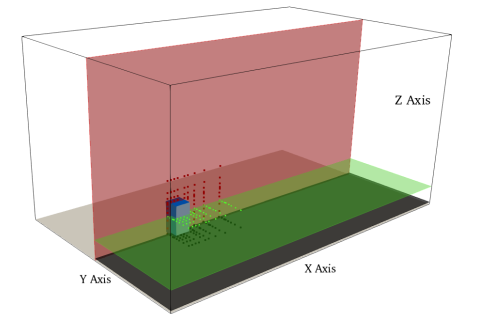
\includegraphics[scale=0.6]{imgs/aij_A.png}
        \caption{Single building immersed in NSBL}
    \end{figure}
    \textbf{Objectives:} 
    \begin{itemize}
        \item grid sensitivity analysis with steady state simulation (standard grid related analysis);
        \item from steady-state simulations to Scale Resolving Simulations (SRS), with kOmegaSSTSAS turbulence model, to highlight differences in terms of accuracy and computational cost (case-specific analysis);
        \item kOmegaSSTSAS turbulence model sensitivity analysis on the grid filter definition (case-specific analysis);
        \item SAS vs LES (case-specific analysis);
        \item development of Adaptive Mesh Refinement (AMR) criteria related to dispersion phenomena (methodology development);
        \item implementation of incremental POD for AMR (feature implementation);
        \item sensitivity analyses on turbulence models, numerical schemes, boundary conditions, and the effects of dimensionality reduction via intrusive ROM (validation-oriented study).
    \end{itemize}
    \textbf{Conclusions:} .... .\newline

\clearpage
\subsubsection{AIJ - Case C - Building blocks immersed in NSBL}
    \begin{figure}[h!]
        \centering
        \hypertarget{link:aij_C}{}
        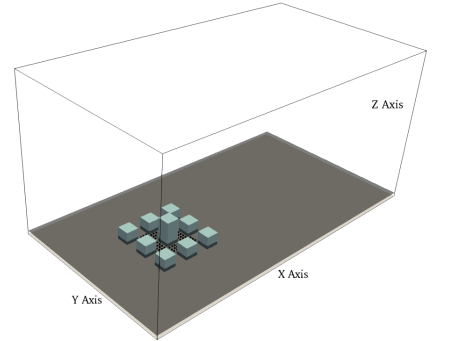
\includegraphics[scale=0.7]{imgs/aij_C.png}
        \caption{Building blocks immersed in NSBL}
    \end{figure}
    \textbf{Objectives:} ....
    \begin{itemize}
        \item grid sensitivity analysis with steady state simulation (standard grid related analysis);
        \item Application of computational methodology defined at the previous step
        \item reduced order modelling with respect changing inflow boundary conditions
        \item sensitivity analyses on turbulence models, numerical schemes, boundary conditions, and the effects of dimensionality reduction via intrusive ROM (validation-oriented study).
    \end{itemize}
    \textbf{Conclusions:} .... .\newline

\clearpage
\subsubsection{SEF - Case A - Street canyon immersed in NSBL}
    \begin{figure}[h!]
        \hypertarget{link:sef_A}{}
        \centering
        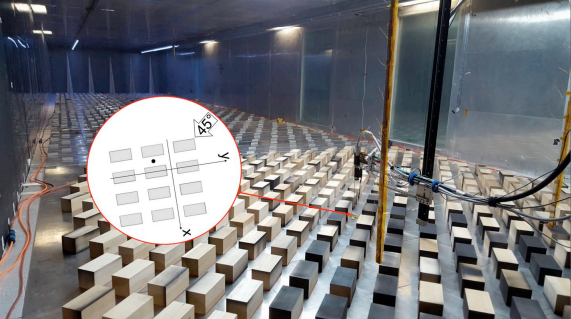
\includegraphics[scale=0.8]{imgs/sef_dataset_image.png}
        \caption{Street canyon immersed in NSBL with and without dispersion
        of heavy gas}
    \end{figure}
    \textbf{Objectives:} ....\newline
    \begin{itemize}
        \item ...
        \item ...
    \end{itemize}
    \textbf{Conclusions:} .... .\newline


\clearpage
\subsubsection{TPU - Case A - Street canyon immersed in NSBL}
    \begin{figure}[h!]
        \hypertarget{link:tpu_A}{}
        \centering
        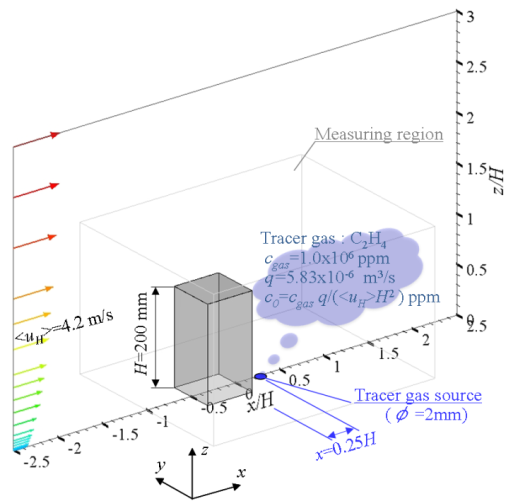
\includegraphics[scale=0.6]{imgs/tpu_dataset_image.png}
        \caption{Street canyon immersed in NSBL with and without dispersion
        of neutral gas}
    \end{figure}
    \textbf{Objectives:} ....\newline
    \begin{itemize}
        \item ...
        \item ...
    \end{itemize}
    \textbf{Conclusions:} .... .\newline

\clearpage
\subsubsection{COST-C-M - Michelstadt dataset - street canyon immersed in NSBL}
    \begin{figure}[h!]
        \hypertarget{link:cost_m}{}
        \centering
        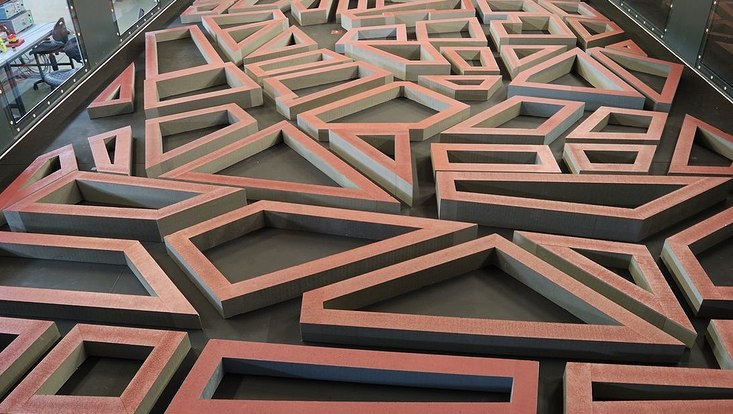
\includegraphics[scale=0.6]{imgs/michelstad.jpg}
        \caption{Street canyon immersed in NSBL}
    \end{figure}
    \textbf{Objectives:} ....\newline
    \begin{itemize}
        \item ...
        \item ...
    \end{itemize}
    \textbf{Conclusions:} .... .\newline

\clearpage
\subsubsection{COST-C-WT - COST ES 1006 CUTE dataset - wind tunnel experiment of a whole city model in NSBL}
    \begin{figure}[h!]
        \hypertarget{link:cost_c_wt}{}
        \centering
        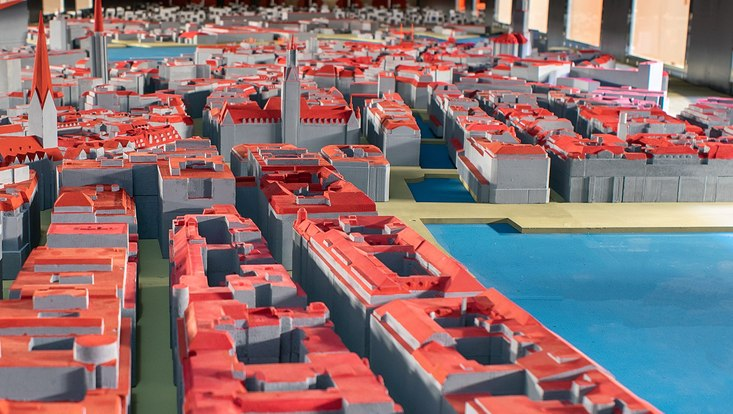
\includegraphics[scale=0.6]{imgs/cute.jpg}
        \caption{Street canyon immersed in NSBL}
    \end{figure}
    \textbf{Objectives:} ....\newline
    \begin{itemize}
        \item ...
        \item ...
    \end{itemize}
    \textbf{Conclusions:} .... .\newline


\clearpage

\subsection{Stable Boundary Layer (SBL)}

\subsubsection{SEF - Case B - Street canyon immersed in SBL}
    \begin{figure}[h!]
        \hypertarget{link:sef_A}{}
        \centering
        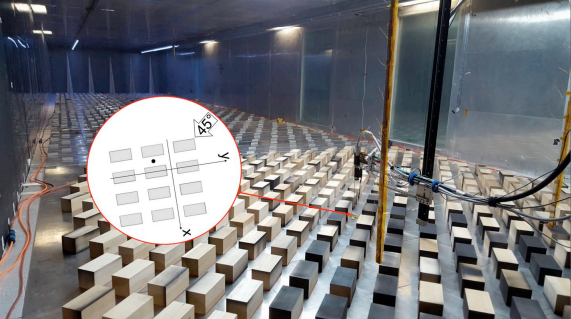
\includegraphics[scale=0.7]{imgs/sef_dataset_image.png}
        \caption{Street canyon immersed in CBL with and without dispersion
        of heavy gas}
    \end{figure}
    \textbf{Objectives:} ....\newline
    \begin{itemize}
    \item ...
    \item ...
    \end{itemize}
    \textbf{Conclusions:} .... .\newline


\clearpage
\subsubsection{TPU - Case B - Street canyon immersed in SBL}
    \begin{figure}[h!]
        \hypertarget{link:tpu_C}{}
        \centering
        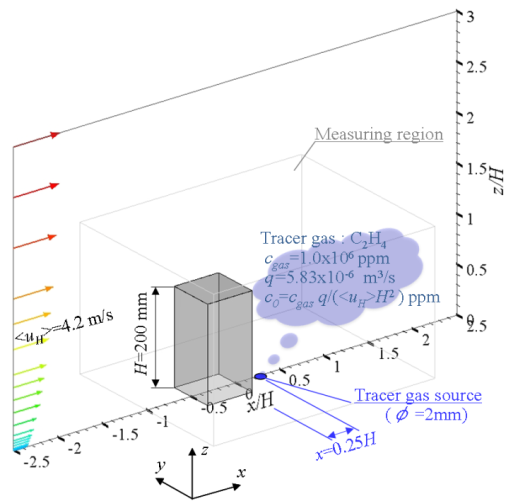
\includegraphics[scale=0.6]{imgs/tpu_dataset_image.png}
        \caption{Street canyon immersed in SBL with dispersion of neutral 
        gas}
    \end{figure}
    \textbf{Objectives:} ....\newline
    \begin{itemize}
        \item ...
        \item ...
    \end{itemize}
    \textbf{Conclusions:} .... .\newline

\clearpage

\subsection{Convective Boundary Layer (CBL)}

\subsubsection{SEF - Case C - Street canyon immersed in CBL}
    \begin{figure}[h!]
        \hypertarget{link:sef_A}{}
        \centering
        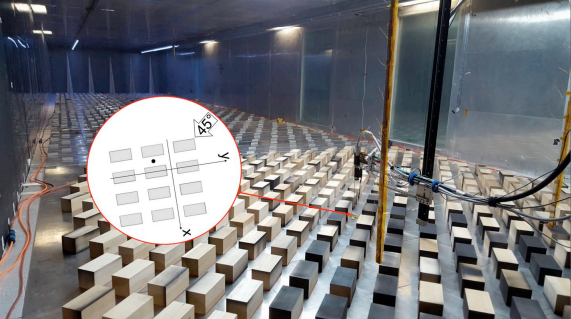
\includegraphics[scale=0.7]{imgs/sef_dataset_image.png}
        \caption{Street canyon immersed in CBL with and without dispersionof heavy gas}
    \end{figure}
    \textbf{Objectives:} ....\newline
    \begin{itemize}
    \item ...
    \item ...
    \end{itemize}
    \textbf{Conclusions:} .... .\newline


\clearpage
\subsubsection{TPU - Case C - Single building immersed in CBL}
    \begin{figure}[h!]
        \hypertarget{link:tpu_C}{}
        \centering
        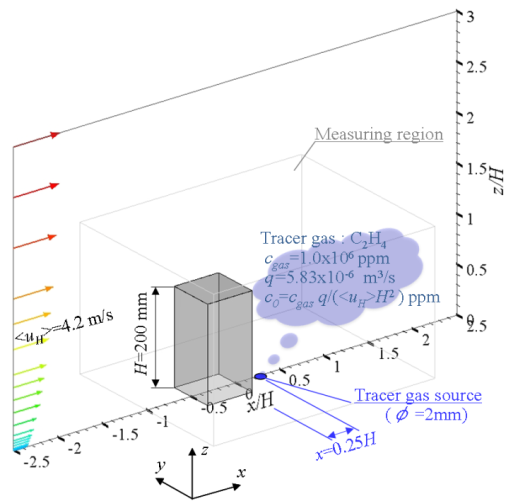
\includegraphics[scale=0.6]{imgs/tpu_dataset_image.png}
        \caption{Street canyon immersed in CBL with dispersion of neutral 
        gas}
    \end{figure}
    \textbf{Objectives:} ....\newline
    \begin{itemize}
        \item ...
        \item ...
    \end{itemize}
    \textbf{Conclusions:} .... .\newline


\clearpage

\subsection{Real-world scenario}

\subsubsection{COST-C-F - COST ES 1006 CUTE dataset - field experiment}
    \begin{figure}[h!]
        \hypertarget{link:cost_c_f}{}
        \centering
        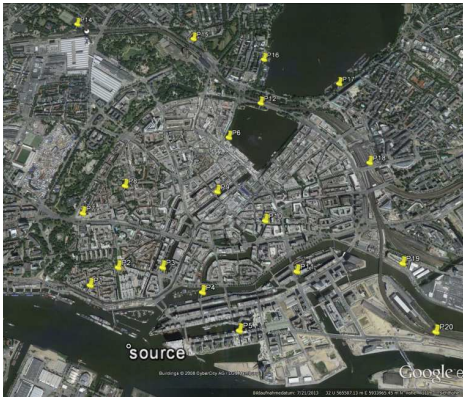
\includegraphics[scale=0.8]{imgs/cute_field_exp.png}
        \caption{Street canyon immersed in CBL with dispersion of neutral 
        gas}
    \end{figure}
    \textbf{Objectives:} ....\newline
    \begin{itemize}
        \item ...
        \item ...
    \end{itemize}
    \textbf{Conclusions:} .... .\newline


\clearpage
\subsubsection{TURB - Prague dataset - Field experiment of Prague}
    \begin{figure}[h!]
        \hypertarget{link:turb_p}{}
        \centering
        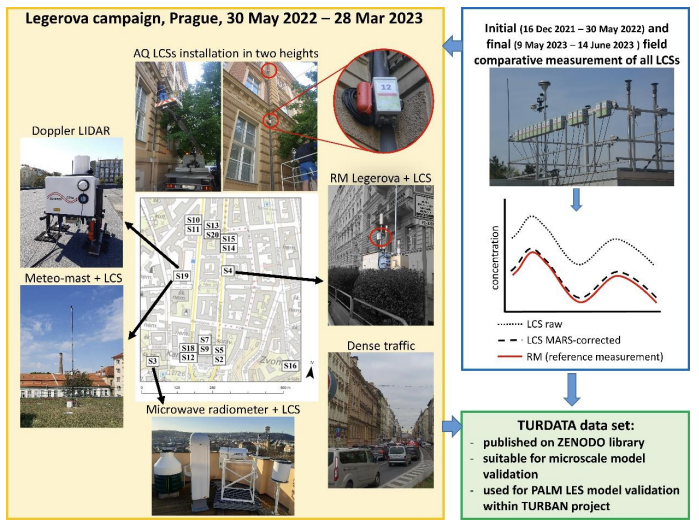
\includegraphics[scale=0.7]{imgs/turban_dataset_image.png}
        \caption{Street canyon immersed in CBL with dispersion of neutral 
        gas}
    \end{figure}
    \textbf{Objectives:} ....\newline
    \begin{itemize}
        \item ...
        \item ...
    \end{itemize}
    \textbf{Conclusions:} .... .\newline


\clearpage


